 -----------------------------------------------------------------------------%
%                            OLD VERSION MANUAL
% -----------------------------------------------------------------------------%

\section{Old Versions Documentation}


\subsection{Manjaro Linux System}

\subsubsection{Creating A Live USB Of Manjaro Linux}
\label{usbLiveCreation}
\par First, please go to 
\href{https://manjaro.org/downloads/official/xfce/}
{manjaro archive download page} and download the "minimal" version ISO of 
Manjaro linux 21.0.
Then, make the ISO file Bootable on USB drive. Under Windows, you
can do it by using \href{https://www.easy2boot.com}{easy2boot} for example. 
Under Linux and Mac, you can use the following instructions.
\newline
\par
Open a terminal, type the following command: 
\begin{lstlisting}[language=commandline]
sudo dmesg -w
\end{lstlisting}

Now connect your USB stick memory, you should get output similar to this:
\begin{lstlisting}[language=commandline, style=output]
[10576.130389] usb-storage 2-6:1.0: USB Mass Storage device detected
[10576.130756] scsi host5: usb-storage 2-6:1.0
[10577.144722] scsi 5:0:0:0: Direct-Access     SanDisk  Ultra USB 3.0    
1.00 PQ: 0 ANSI: 6
[10577.145229] sd 5:0:0:0: Attached scsi generic sg6 type 0
[10577.145493] sd 5:0:0:0: [sdf] 30031872 512-byte logical blocks: 
(15.4 GB/14.3 GiB)
[10577.146230] sd 5:0:0:0: [sdf] Write Protect is off
[10577.146233] sd 5:0:0:0: [sdf] Mode Sense: 43 00 00 00
[10577.146485] sd 5:0:0:0: [sdf] Write cache: disabled, read cache: 
enabled, doesn't support DPO or FUA
[10577.153805]  sdf: sdf1
[10577.155586] sd 5:0:0:0: [sdf] Attached SCSI removable disk
\end{lstlisting}

Here, the linux device naming for the USB key is \emph{/dev/sdf} (line 12).
Next step is to \emph{unmount} all file systems of this USB key from
the file hierarchy in order to prevent any access by other application.
Then we need to format the unmounted drive in Linux jounaling file system
\emph{ext4}.
And finally copy the Manjaro Linux ISO file to the USB drive.
Adapt the following commands with the name of your device and the path to the
ISO file you just downloaded. Note the ending star for the first command.

\vspace{6pt}
\textbf{\textcolor{red}{Warning: it is critically important not to copy the ISO onto the
wrong device! Please double check before going ahead with the next.}}

\begin{lstlisting}
umount /dev/sdf*
sudo dd if=/path/to/manjaro.iso of=/dev/sdf status="progress"
\end{lstlisting}
If ISO is properly copied to bootable USB, you should see the new name 
MJRO1815 for the USB key.

% -----------------------------------------------------------------------------%
\subsubsection{Install and Update Manjaro Linux}
Insert the Live USB flash drive into the computer, power it, and get access to the
BIOS (see annex \ref{annex:bios}). Go under the tab named \emph{Boot} and press enter 
on the menu \emph{Hard Drive BBS Priorities}. You should see the name of your hard-drive 
on the first row and the name of your usb drive on the second one. If you don't see your 
USB key in here this may mean your bootable USB key is not made properly.
Use \textbf{\textless+/-\textgreater} controls to put your flash drive on the first, 
then press \textbf{\textless Esc\textgreater} to quit the menu, go under 
\emph{Save \& Exit} and select \emph{Save Changes and Reset}.
% Note : BBS = BIOS Boot Specification
\newline
\par

\begin{minipage}[c]{0.15\textwidth}
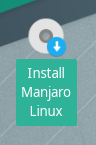
\includegraphics[width=\textwidth]{images/manjaro0.png}
\end{minipage}
\hfill
\begin{minipage}[c]{0.75\textwidth}
Once Manjaro has started, double-click on the icon \emph{Install Manjaro Linux}
(lower left corner)
\begin{itemize}
	\item Use American English (US)
	\item Choose Europe as Region and London as Zone
	\item Choose ERASE DISK
	\item Login and password (use same for administrator)
\end{itemize}
\end{minipage}
\par
\vspace{11pt}
Then reboot again without the USB stick. After getting your desktop environment 
started, set up an Internet connection, open a terminal (press 
\textbf{\textless ctrl + alt + t \textgreater}) and type the following commands
in the terminal in order to clean your \textit{home directory} 
update the system and install \textit{git}:
\begin{lstlisting}
rmdir Music/ Pictures/ Videos/ Public/ Templates/
sudo pacman -Syu
sudo pacman -S git
sudo pacman -S git
\end{lstlisting}

\noindent Say yes/or default [ENTER] to all questions. Note that once done, the computer may 
reboot.

\clearpage

\subsection{Wi-Fi Connection Between the Yocto-Pictor and the rugged PC}
\timeclock{0}{10}
\vspace{16pt}

The Yocto-Pictor, provided as the electronic card of Hypernets system is
controlled through Wi-Fi by the rugged PC. The three following subsections
describe how to set-up this communication.

\subsubsection{Wi-Fi Hotspot Set-up}
\label{sec:wifirugged}
\par
This part aims to configure the Wi-Fi of the rugged PC. It will mainly be used
to control the Yocto-Pictor. But will also be useful to access the rugged PC
after having installed it in the main box of the system.

\begin{itemize}
	\item First, right click on the the connection logo in the bottom right corner of the
screen and click \emph{Edit Connections...} (see figure \ref{fig:editConnection}). 
	\item Click on  \textbf{+}  to add a new connection and select \emph{Wi-Fi} for the 
		Connection Type. 

		On the tab \emph{General}:
		\begin{itemize}
			\item Check \emph{Connect automatically with priority 1}
			\item Check \emph{All users may connect to this network}
		\end{itemize}

		On the tab \emph{Wi-Fi}:
		\begin{itemize}
			\item Set the mode to \emph{Hotspot}
			\item Choose a \emph{SSID}: the name that will appear as Wi-Fi network. 
		\end{itemize}

		On the tab \emph{Wi-Fi Security} (see figure \ref{fig:wifiConfig}).
		\begin{itemize}
			\item Set the security to \emph{WPA \& WPA2 Personal}, 
			\item Choose a valid password
		\end{itemize}
		\item Choose a connection name (on the very top)
		\item Save 
		\item Close the current window and finally left click on 
			the connection logo, \emph{Create New Wi-Fi Network} 
			(see figure \ref{fig:retrieveWifi})
			and select your connection in the drop-down list to enable it.
			
\end{itemize}


\textbf{Note:} further, you may want to use Wi-Fi connection to get an
internet acces. Keep in mind that you can switch the Wi-Fi connection and 
get back to the previous one by following this last step.


\begin{figure}[H]
	\centering
	\begin{minipage}[l]{0.49\linewidth}
		\centering
		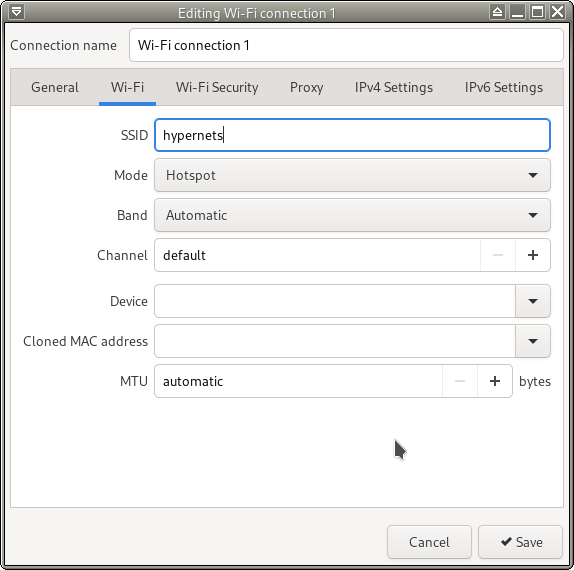
\includegraphics[width=\linewidth]{images/wifi2.png}
		\caption{Edit Connections}
		\label{fig:editConnection}
	\end{minipage}
	\begin{minipage}[r]{0.49\linewidth}
		\centering
		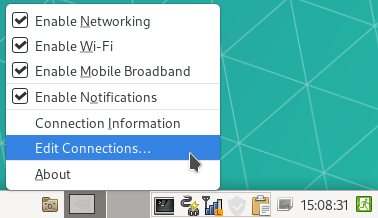
\includegraphics[width=.8\linewidth]{images/wifi1.png}
		\caption{Wi-Fi Connections Access}
		\label{fig:wifiConfig}
		\vspace{\baselineskip}
		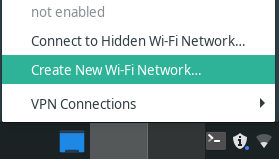
\includegraphics[width=.7\linewidth]{images/wifi3.png}
		\caption{Retrieve Wi-Fi Hotspot} \par
		\label{fig:retrieveWifi}
	\end{minipage}
\end{figure}


% -----------------------------------------------------------------------------%
\subsubsection{Setting up the Yoctopuce VirtualHub}
\label{sec:virtualhub}
% \timeclock{0}{10}
% \newline
\par 
According to the \href{https://www.yoctopuce.com/EN/virtualhub.php}{Yoctopuce
documentation}: 
\begin{quotation}
The VirtualHub is a toolbox for Yoctopuce USB devices. It will allow you
to:
	\begin{itemize}
	 \item configure and test Yoctopuce devices
	 \item remotely control Yoctopuce devices through network
	\end{itemize}
\end{quotation}

Here, you should have an updated linux distribution on your rugged PC and
a working internet connection wired on it.
Open a terminal, clone the installation script repository on your home folder,
and run the script with \emph{sudo priveleges}:

% git clone --recurse-submodules https://github.com/hypernets/hypernets_tools
\begin{lstlisting}
<ctrl + alt + t>  # open a terminal
cd
git clone https://github.com/hypernets/hypernets_tools
git checkout beta
cd hypernets_tools/
sudo ./install/00_install_yoctohub.sh
\end{lstlisting}
You should now be able to run the VirtualHub by typing:
\begin{lstlisting}
/usr/sbin/VirtualHub
\end{lstlisting}

% -----------------------------------------------------------------------------%
\subsubsection{Yocto-Pictor Wi-Fi Connection}
\label{sec:yocto-wifi}
\par
Run the VirtualHub (see last command in the previous section), 
open the web browser and visit the following address:
\begin{lstlisting}
127.0.0.1:4444
\end{lstlisting}
\par
If you don't see a screen like figure \ref{fig:screenyocto}, please retry 
instructions from the above section \pageref{sec:virtualhub}. 

If you were using Wi-Fi to get Internet, enable the hotspot (see last note from
section \pageref{sec:wifirugged})

Plug the Wi-Fi antenna (see figure \ref{fig:yoctoAntenna}) and connect the
Yocto-Pictor-Wifi with your usb cable on the config port (see figure \ref{fig:yoctoUSBtop}). 
Click on the button \emph{configure} and edit the \emph{WLAN settings} in the section 
\emph{Network Configuration}: 
\begin{enumerate}
		\item Select \emph{Infrastructure (choose an existing WLAN)}.
		\item Enter the password you choose in section \pageref{sec:wifirugged}.
		\item Click on \emph{Test Config} and note the displayed Current IP.
		\item Save and exit.
\end{enumerate}

Now, you can come back to your terminal with \textbf{\textless ctrl + alt + t \textgreater}
and quit the VirtualHub \textbf{\textless ctrl + c \textgreater}.

Type the IP address followed by \emph{":4444"} in the address bar of the web browser 
and you should see a screen similar to the one before with 3 lines and serials 
(see figure \ref{fig:yoctoSerial}). Note the 3 serials of these devices and the IP address. 
It will be required later (in the section \pageref{sec:yocto-config}).
\vspace{11pt}

\emph{Note: at this point you should consider to update the firmwares (see the
annex \ref{annex:yoctoUpdate})}

\begin{figure}[!ht]
  \centering
  \begin{minipage}[b]{0.35\textwidth}
	  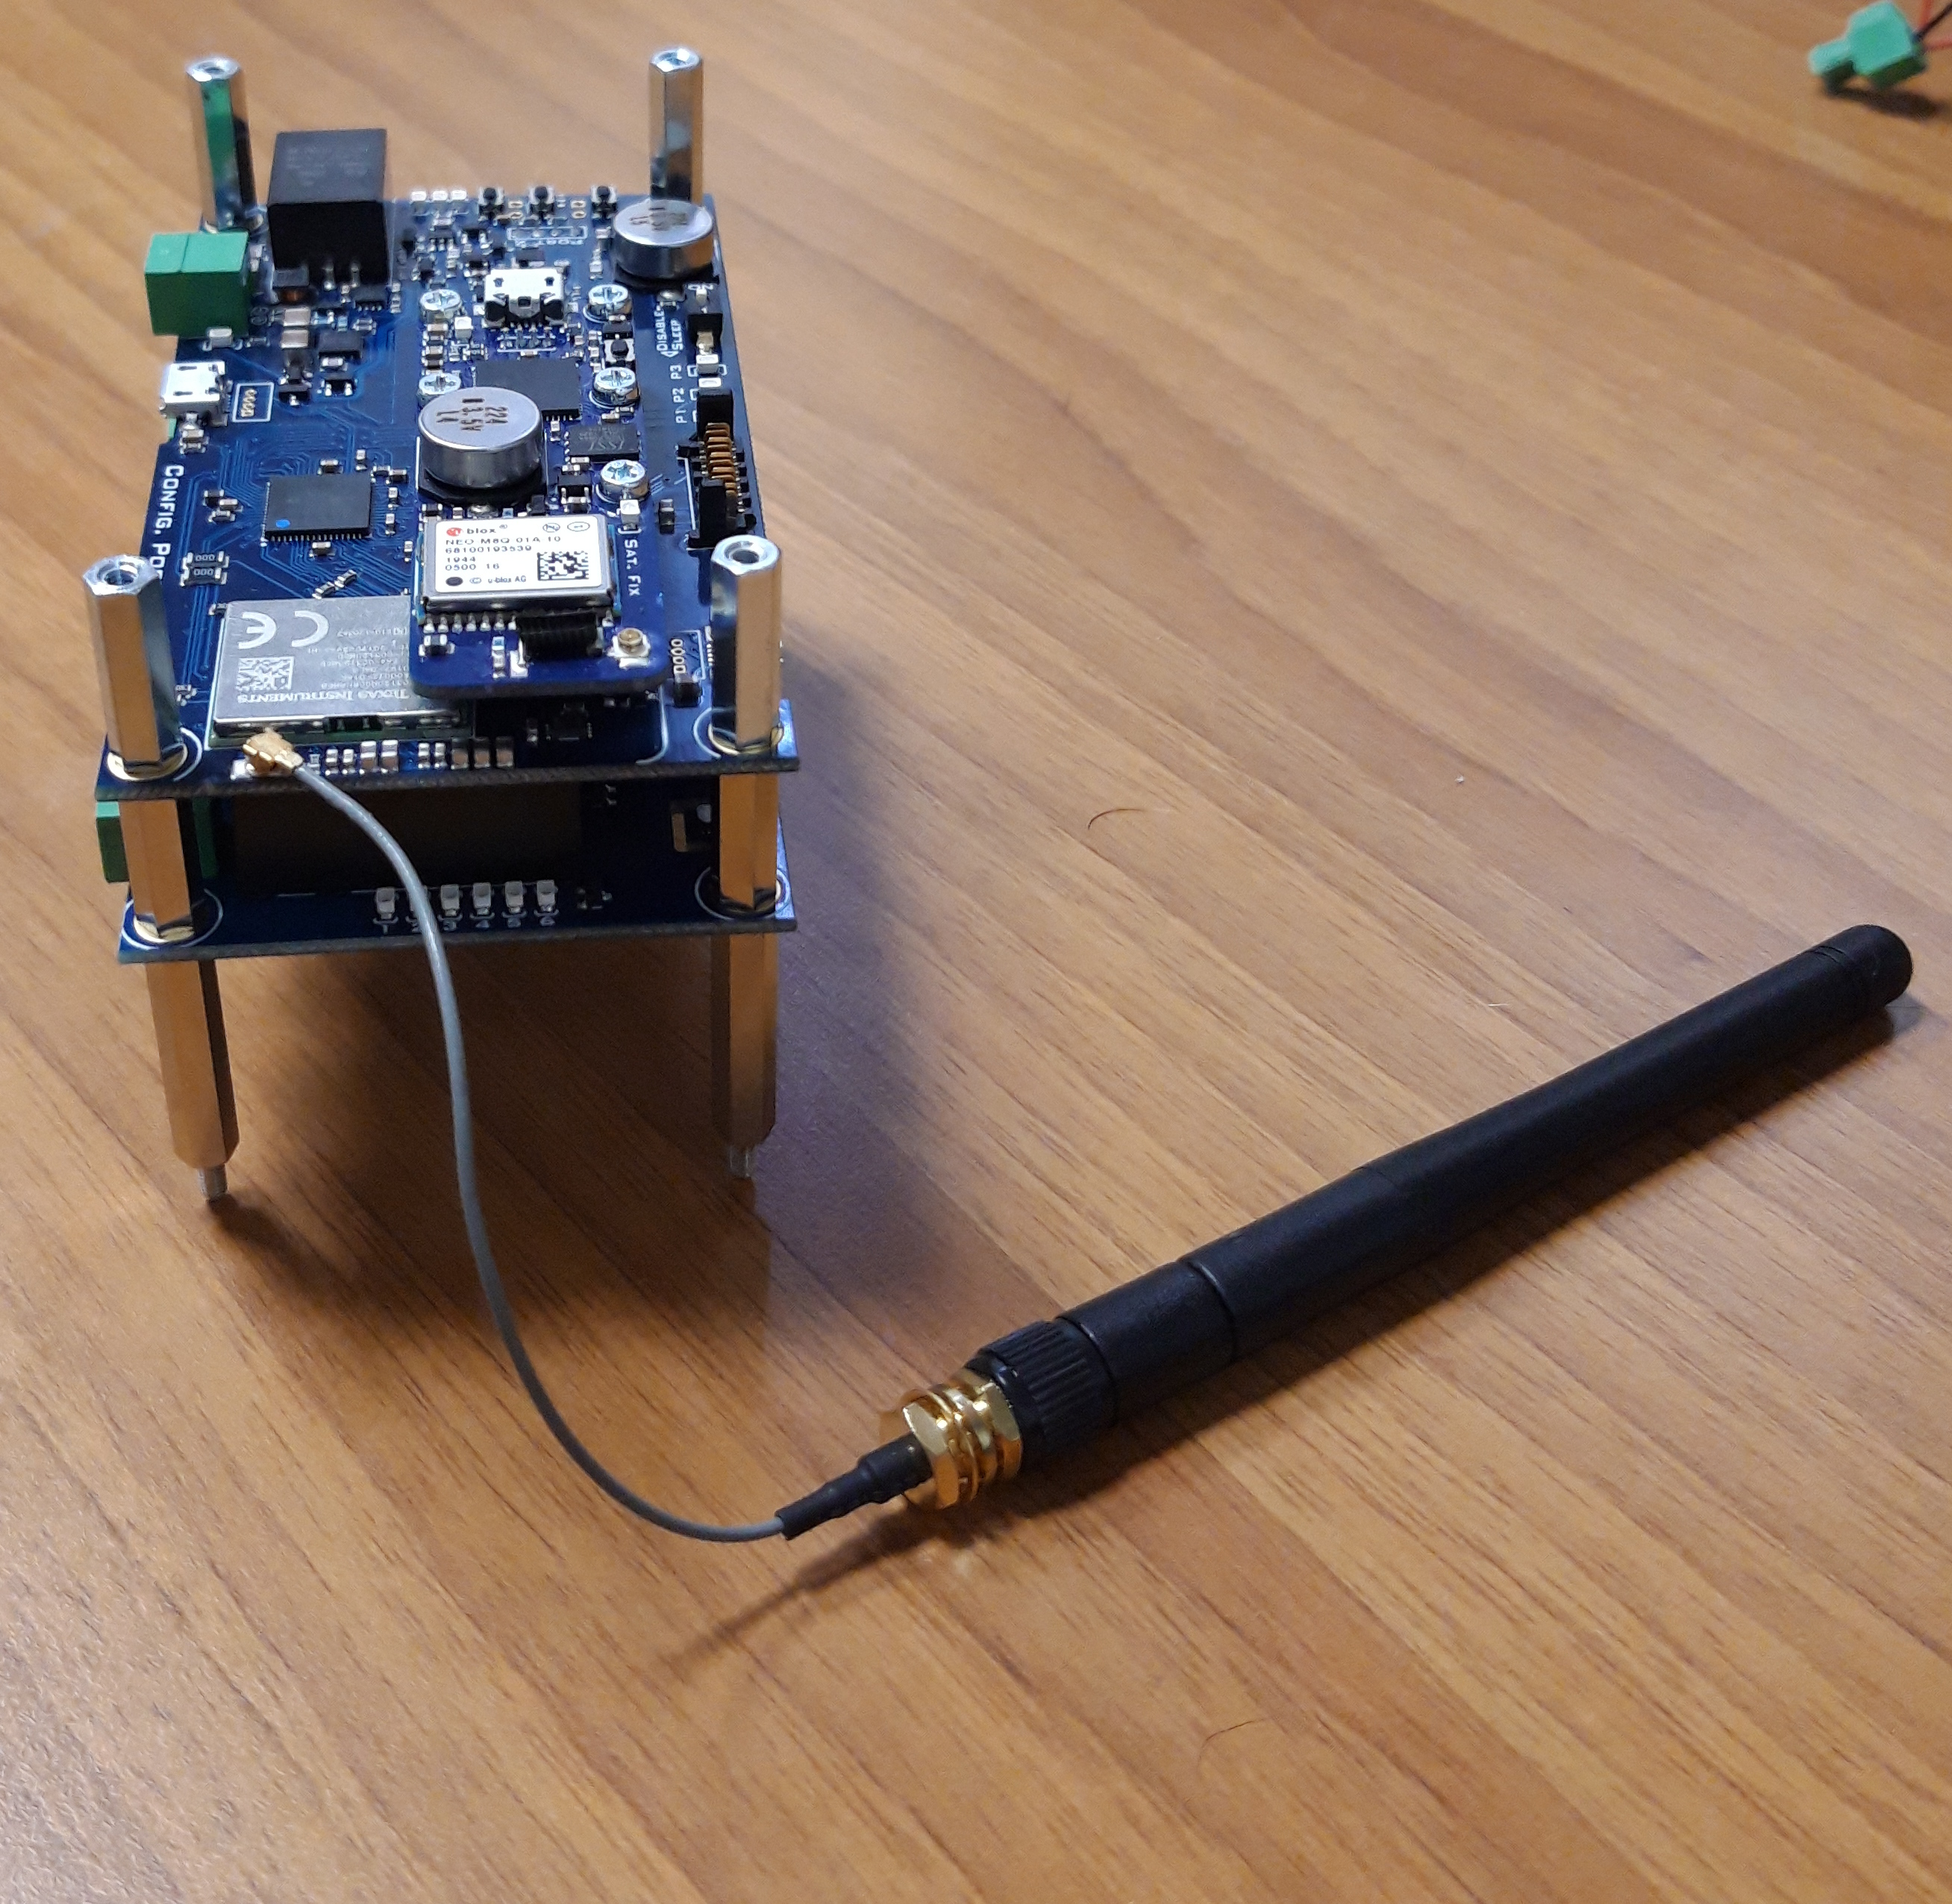
\includegraphics[width=\linewidth]{images/yoctopuce_wifi.jpg}
	\caption{Wi-Fi Antenna}
	\label{fig:yoctoAntenna}
  \end{minipage}
  \hfill
  \begin{minipage}[b]{0.55\textwidth}
	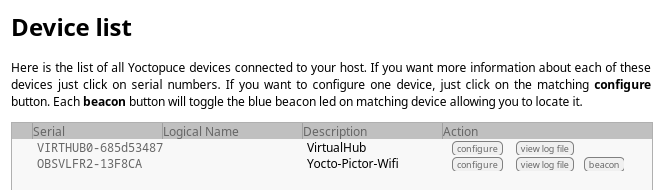
\includegraphics[width=\linewidth]{images/yocto1.png}
    \caption{Web Interface: Virtual Hub}
	\label{fig:screenyocto}
  \end{minipage}
\end{figure}

\begin{figure}[!ht]
  \centering
  \begin{minipage}[b]{0.35\textwidth}
	\includegraphics[width=\linewidth]{images/yoctopuce_usb2.jpg}
	  \vspace{11pt}
	\caption{Yocto-Pictor: top floor USB connection}
	\label{fig:yoctoUSBtop}
  \end{minipage}
  \hfill
  \begin{minipage}[b]{0.55\textwidth}
	  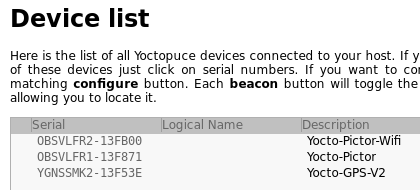
\includegraphics[width=\linewidth]{images/yocto3.png}
	\caption{Web Interface: serial}
	\label{fig:yoctoSerial}
  \end{minipage}
\end{figure}

\subsection{Linking Hypernets Tools to the Yocto-Pictor}

\label{sec:yocto-config}
If not already done, first copy the two configuration file templates in 
the hypernets\_tools folder:

\begin{lstlisting}
cd hypernets_tools/
cp hypernets/resources/config_dynamic.ini.template config_dynamic.ini
cp hypernets/resources/config_static.ini.template config_static.ini
\end{lstlisting}

Connect the PC to the internet, go to the folder \emph{hypernets\_tools} and 
install required dependencies:

\begin{lstlisting}
cd hypernets_tools/
sudo ./install/01_dependencies.sh
\end{lstlisting}

Now copy the template of the static configuration file 
(see description in annex \ref{annex:staticconfig}) and edit the Yoctopuce
section according to the serial that you previously noted in the section 
\pageref{sec:yocto-wifi}:

\begin{lstlisting}
cp hypernets/resources/static_config.ini.template static_config.ini
mousepad static_config.ini
\end{lstlisting}


If necessary, mind to switch back the Wi-Fi connection to the hotspot mode
(\ref{sec:wifirugged}) and try to run the Graphical User Interface (GUI) with: 

\begin{lstlisting}
python -m hypernets.gui.frame_yoctopuce
\end{lstlisting}

You should see some meteo and GPS data after clicking on \emph{Connection}. 
Also you can try playing with relays to check if everything is working 
(see figure \ref{gui_yocto}).


\begin{figure}[!ht]
	\centering
	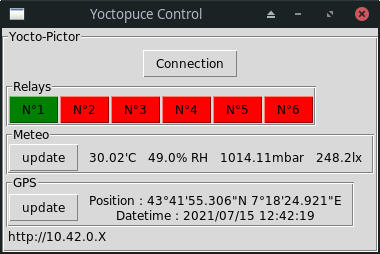
\includegraphics[scale=.55]{images/gui_yocto.png}
	\caption{GUI Yoctopuce Control}
	\label{gui_yocto}
\end{figure}


\subsubsection{Radiometer Configuration and First tests with the GUI}
\begin{itemize}
	\item Yocto-Pictor
	\item USB 2.0 cable of type A-micro B (data + power) 
\end{itemize}

Open a terminal and type the following command in order to link the radiometer
to a \textit{device file}:
\begin{lstlisting}
sudo ./install/02_configure_ports.sh
\end{lstlisting}
This should output with something like:
\begin{lstlisting}
lrwxrwxrwx 1 root root 7 Jul 15 15:04 /dev/radiometer0 -> ttyUSB5
\end{lstlisting}
Type the following command (required internet connection) to update the
\textit{libhypstar driver}:
\begin{lstlisting}
sudo ./install/03_update_libhypstar.sh
\end{lstlisting}
